\section{Optimierung}\label{optimierung}

\textbf{Sequentiell, ohne \texttt{-fopenmp}:}

\texttt{./partdiff-seq 1 2 512 2 2 200} braucht \textbf{120.29s}.

\textbf{1 Thread, mit \texttt{-fopenmp}:}

\texttt{./partdiff-seq 1 2 512 2 2 200} braucht \textbf{120.65s}.

\textbf{12 Threads, mit \texttt{-fopenmp}:}

\texttt{./partdiff-seq 1 2 512 2 2 200} braucht \textbf{14.9s}.

\textbf{Mit verschiedenen Schedulings, jw 12 Threads:}

\begin{itemize}
\itemsep1pt\parskip0pt\parsep0pt
\item
  \textbf{\texttt{schedule(dynamic, 1)}:}

  \begin{itemize}
  \itemsep1pt\parskip0pt\parsep0pt
  \item
    \texttt{./partdiff-seq 1 2 512 2 2 200} braucht \textbf{11.39s}.
  \item
    Speedup zu ohne OMP: \textbf{10.59}. The winner! :)
  \end{itemize}
\item
  \textbf{\texttt{schedule(dynamic, 4)}:}

  \begin{itemize}
  \itemsep1pt\parskip0pt\parsep0pt
  \item
    \texttt{./partdiff-seq 1 2 512 2 2 200} braucht \textbf{14.2s}.
  \item
    Speedup zu ohne OMP: \textbf{\textasciitilde{}8.5}.
  \end{itemize}
\item
  \textbf{\texttt{schedule(guided)}:}

  \begin{itemize}
  \itemsep1pt\parskip0pt\parsep0pt
  \item
    \texttt{./partdiff-seq 1 2 512 2 2 200} braucht \textbf{12.3s}.
  \item
    Speedup zu ohne OMP: \textbf{9.8}.
  \end{itemize}
\item
  \textbf{\texttt{schedule(static, 1)}:}

  \begin{itemize}
  \itemsep1pt\parskip0pt\parsep0pt
  \item
    \texttt{./partdiff-seq 1 2 512 2 2 200} braucht \textbf{14.1s}.
  \end{itemize}
\item
  \textbf{\texttt{schedule(static, 2)}:}

  \begin{itemize}
  \itemsep1pt\parskip0pt\parsep0pt
  \item
    \texttt{./partdiff-seq 1 2 512 2 2 200} braucht \textbf{14.7s}.
  \end{itemize}
\item
  \textbf{\texttt{schedule(static, 16)}:}

  \begin{itemize}
  \itemsep1pt\parskip0pt\parsep0pt
  \item
    \texttt{./partdiff-seq 1 2 512 2 2 200} braucht \textbf{14.57s}.
  \end{itemize}
\end{itemize}

Zeit benötigt: 2h. Fehlersuche? Ja, zuerst haben wir die simple
interference function geenommen und dadurch nur ein Speedup von 4
erreicht.

\section{Messungen}\label{messungen}

\subsection{Messung 1}\label{messung-1}

\begin{longtable}[c]{@{}lll@{}}
\toprule
procs & speedup & time in sec\tabularnewline
\midrule
\endhead
1 (no OMP) & 1 & 120.29\tabularnewline
1 & 1 & 120.65\tabularnewline
2 & 2.044222298 & 59.02\tabularnewline
3 & 2.960009814 & 40.76\tabularnewline
4 & 4.045942321 & 29.82\tabularnewline
5 & 4.868845843 & 24.78\tabularnewline
6 & 5.952146029 & 20.27\tabularnewline
7 & 6.710233593 & 17.98\tabularnewline
8 & 7.65060241 & 15.77\tabularnewline
9 & 8.431167016 & 14.31\tabularnewline
10 & 9.1332324 & 13.21\tabularnewline
11 & 9.913722268 & 12.17\tabularnewline
12 & 9.995857498 & 12.07\tabularnewline
\bottomrule
\end{longtable}

\begin{figure}[htbp]
\centering
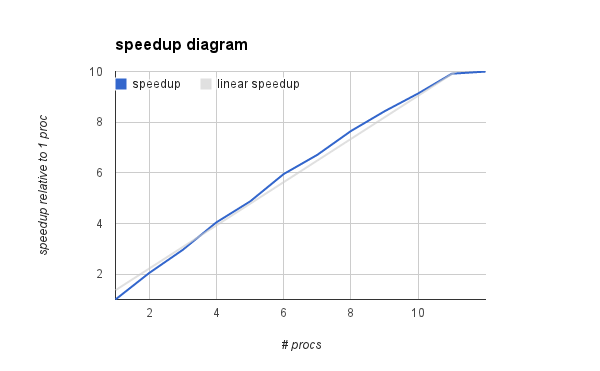
\includegraphics{speedup.png}
\caption{}
\end{figure}
